\section{In-depth analysis}
In this section we perform an in-depth analysis of the performance of the CLM and C&M2020 methods when changing the control chart design parameter.
Herein, the OC performance of the proposed cautious learning parameter update rules are compared to the fixed and adaptive estimators.
We use the same simulation settings as in Section ?? of the paper regarding the intial sample size, cautious learning parameters, parameter shift magnitude and location, and control limit design.
The IC process parameter is fixed to $\theta = 4$ and we study the performance of the proposed methodology as $ \lambda$ varies in $\{0.05, 0.075, 0.1, 0.125, 0.15, 0.175, 0.2\} $.
From the results in \Cref{fig:lambda=0.05/EWMA OC theta=4,fig:lambda=0.075/EWMA OC theta=4,fig:lambda=0.10/EWMA OC theta=4,fig:lambda=0.125/EWMA OC theta=4,fig:lambda=0.15/EWMA OC theta=4,fig:lambda=0.175/EWMA OC theta=4,fig:lambda=0.20/EWMA OC theta=4}, it is possible to see that the parameter estimator based on time-delayed update rules provide consistently improved results when compared to both adaptive and fixed estimators.
This appears to be valid across both shift sizes and control chart design parameter, with differences between the \textit{CLM and the C\&M2020 approaches}.
Overall, the suggested settings of $ A=1.5$ and $ B=50$ for the \textit{C\&M2020} update rule results in a more conservative update rule than the CLM approach.
Indeed, when the control chart displays a high sensitivity to small shifts such as in \Cref{fig:lambda=0.05/EWMA OC theta=4}, the CLM approach provides a protection against early shifts that is comparable to the \textit{C\&M2020} update rule.
However, the CLM approach provides a better protection to shifts that happen later in the monitoring phase due to the higher precision of the estimates.
Conversely, when the control chart is less sensitive to small parameter shifts (\Cref{fig:lambda=0.20/EWMA OC theta=4}), the conservativeness of the \textit{C\&M2020} approach is better apt at detecting early parameter shifts.
Overall, among the proposed delayed-parameter update rules we do not observe a clear winner, since the performance seems to depend on the sensitivity of the control chart to smaller or larger shifts.
Finally, the proposed delayed estimators appear to provide a better overall performance than the fully adaptive estimator, which shows degraded detection power when $ \tau=1$.

% --- Lambda = 0.05

% \begin{figure}
% \centering
% \begin{subfigure}{0.49\textwidth}
%   \centering
%   \caption{$ \delta = 0.25$}
%   \label{fig:lambda=0.05/theta=4.0/delta=0.25}
%   \includegraphics[width=\textwidth]{figures/sims/theta=4.0_signedEWMA(l = 0.05, upw = true, L = 1.0)/delta=0.25.png}
% \end{subfigure}
% \begin{subfigure}{0.49\textwidth}
%   \centering
%   \caption{$ \delta = 0.35$}
%   \label{fig:lambda=0.05/theta=4.0/delta=0.35}
%   \includegraphics[width=\textwidth]{figures/sims/theta=4.0_signedEWMA(l = 0.05, upw = true, L = 1.0)/delta=0.35.png}
% \end{subfigure}
% \begin{subfigure}{0.49\textwidth}
%   \centering
%   \caption{$ \delta = 0.5$}
%   \label{fig:lambda=0.05/theta=4.0/delta=0.5}
%   \includegraphics[width=\textwidth]{figures/sims/theta=4.0_signedEWMA(l = 0.05, upw = true, L = 1.0)/delta=0.50.png}
% \end{subfigure}
% \begin{subfigure}{0.49\textwidth}
%   \centering
%   \caption{$ \delta = 0.75$}
%   \label{fig:lambda=0.05/theta=4.0/delta=0.75}
%   \includegraphics[width=\textwidth]{figures/sims/theta=4.0_signedEWMA(l = 0.05, upw = true, L = 1.0)/delta=0.75.png}
% \end{subfigure}
% \begin{subfigure}{0.49\textwidth}
%   \centering
%   \caption{$ \delta = 1.0$}
%   \label{fig:lambda=0.05/theta=4.0/delta=1.0}
%   \includegraphics[width=\textwidth]{figures/sims/theta=4.0_signedEWMA(l = 0.05, upw = true, L = 1.0)/delta=1.00.png}
% \end{subfigure}
% \begin{subfigure}{0.49\textwidth}
%   \centering
%   \caption{$ \delta = 1.25$}
%   \label{fig:lambda=0.05/theta=4.0/delta=1.25}
%   \includegraphics[width=\textwidth]{figures/sims/theta=4.0_signedEWMA(l = 0.05, upw = true, L = 1.0)/delta=1.25.png}
% \end{subfigure}
%   \caption{OC performance of the EWMA ($ \lambda = 0.05$) control chart under fixed (FE), adaptive (AE), and cautious learning (CL) parameter updates when $ \gj = 4$.
%     Control charts satisfy the GICP condition \eqref{eq:GICP} with $ \beta = 0.1$.
%   Boxplots are based on the 200 simulated conditional ARLs.}
%   \label{fig:lambda=0.05/EWMA OC theta=4}
% \end{figure}

% \begin{figure}
%   \includegraphics[width=\textwidth]{figures/sims/theta=4.0_signedEWMA(l = 0.05, upw = true, L = 1.0)/OC-profiles.png}
%   \caption{Median of the OC conditional ARL of the EWMA-type control chart under fixed (FE), adaptive (AE), cautious learning (CL) parameter updates for $ \gj = 4$ and $ \lambda = 0.05$.
%     Control charts satisfy the GICP condition \eqref{eq:GICP} with $ \beta = 0.1$.
%   Plots are based on the 200 simulated conditional ARLs.}
%   \label{fig:lambda=0.05/EWMA OC profiles}
% \end{figure}

% --- Lambda = 0.075

% \begin{figure}
% \centering
% \begin{subfigure}{0.49\textwidth}
%   \centering
%   \caption{$ \delta = 0.25$}
%   \label{fig:lambda=0.075/theta=4.0/delta=0.25}
%   \includegraphics[width=\textwidth]{figures/sims/theta=4.0_signedEWMA(l = 0.075, upw = true, L = 1.0)/delta=0.25.png}
% \end{subfigure}
% \begin{subfigure}{0.49\textwidth}
%   \centering
%   \caption{$ \delta = 0.35$}
%   \label{fig:lambda=0.075/theta=4.0/delta=0.35}
%   \includegraphics[width=\textwidth]{figures/sims/theta=4.0_signedEWMA(l = 0.075, upw = true, L = 1.0)/delta=0.35.png}
% \end{subfigure}
% \begin{subfigure}{0.49\textwidth}
%   \centering
%   \caption{$ \delta = 0.5$}
%   \label{fig:lambda=0.075/theta=4.0/delta=0.5}
%   \includegraphics[width=\textwidth]{figures/sims/theta=4.0_signedEWMA(l = 0.075, upw = true, L = 1.0)/delta=0.50.png}
% \end{subfigure}
% \begin{subfigure}{0.49\textwidth}
%   \centering
%   \caption{$ \delta = 0.75$}
%   \label{fig:lambda=0.075/theta=4.0/delta=0.75}
%   \includegraphics[width=\textwidth]{figures/sims/theta=4.0_signedEWMA(l = 0.075, upw = true, L = 1.0)/delta=0.75.png}
% \end{subfigure}
% \begin{subfigure}{0.49\textwidth}
%   \centering
%   \caption{$ \delta = 1.0$}
%   \label{fig:lambda=0.075/theta=4.0/delta=1.0}
%   \includegraphics[width=\textwidth]{figures/sims/theta=4.0_signedEWMA(l = 0.075, upw = true, L = 1.0)/delta=1.00.png}
% \end{subfigure}
% \begin{subfigure}{0.49\textwidth}
%   \centering
%   \caption{$ \delta = 1.25$}
%   \label{fig:lambda=0.075/theta=4.0/delta=1.25}
%   \includegraphics[width=\textwidth]{figures/sims/theta=4.0_signedEWMA(l = 0.075, upw = true, L = 1.0)/delta=1.25.png}
% \end{subfigure}
%   \caption{OC performance of the EWMA ($ \lambda = 0.075$) control chart under fixed (FE), adaptive (AE), and cautious learning (CL) parameter updates when $ \gj = 4$.
%     Control charts satisfy the GICP condition \eqref{eq:GICP} with $ \beta = 0.1$.
%   Boxplots are based on the 200 simulated conditional ARLs.}
%   \label{fig:lambda=0.075/EWMA OC theta=4}
% \end{figure}

% \begin{figure}
%   \includegraphics[width=\textwidth]{figures/sims/theta=4.0_signedEWMA(l = 0.075, upw = true, L = 1.0)/OC-profiles.png}
%   \caption{Median of the OC conditional ARL of the EWMA-type control chart under fixed (FE), adaptive (AE), cautious learning (CL) parameter updates for $ \gj = 4$ and $ \lambda = 0.075$.
%     Control charts satisfy the GICP condition \eqref{eq:GICP} with $ \beta = 0.1$.
%   Plots are based on the 200 simulated conditional ARLs.}
%   \label{fig:lambda=0.05/EWMA OC profiles}
% \end{figure}

% --- Lambda = 0.1

% \begin{figure}
% \centering
% \begin{subfigure}{0.49\textwidth}
%   \centering
%   \caption{$ \delta = 0.25$}
%   \label{fig:lambda=0.10/theta=4.0/delta=0.25}
%   \includegraphics[width=\textwidth]{figures/sims/theta=4.0_signedEWMA(l = 0.1, upw = true, L = 1.0)/delta=0.25.png}
% \end{subfigure}
% \begin{subfigure}{0.49\textwidth}
%   \centering
%   \caption{$ \delta = 0.35$}
%   \label{fig:lambda=0.10/theta=4.0/delta=0.35}
%   \includegraphics[width=\textwidth]{figures/sims/theta=4.0_signedEWMA(l = 0.1, upw = true, L = 1.0)/delta=0.35.png}
% \end{subfigure}
% \begin{subfigure}{0.49\textwidth}
%   \centering
%   \caption{$ \delta = 0.5$}
%   \label{fig:lambda=0.10/theta=4.0/delta=0.5}
%   \includegraphics[width=\textwidth]{figures/sims/theta=4.0_signedEWMA(l = 0.1, upw = true, L = 1.0)/delta=0.50.png}
% \end{subfigure}
% \begin{subfigure}{0.49\textwidth}
%   \centering
%   \caption{$ \delta = 0.75$}
%   \label{fig:lambda=0.10/theta=4.0/delta=0.75}
%   \includegraphics[width=\textwidth]{figures/sims/theta=4.0_signedEWMA(l = 0.1, upw = true, L = 1.0)/delta=0.75.png}
% \end{subfigure}
% \begin{subfigure}{0.49\textwidth}
%   \centering
%   \caption{$ \delta = 1.0$}
%   \label{fig:lambda=0.10/theta=4.0/delta=1.0}
%   \includegraphics[width=\textwidth]{figures/sims/theta=4.0_signedEWMA(l = 0.1, upw = true, L = 1.0)/delta=1.00.png}
% \end{subfigure}
% \begin{subfigure}{0.49\textwidth}
%   \centering
%   \caption{$ \delta = 1.25$}
%   \label{fig:lambda=0.10/theta=4.0/delta=1.25}
%   \includegraphics[width=\textwidth]{figures/sims/theta=4.0_signedEWMA(l = 0.1, upw = true, L = 1.0)/delta=1.25.png}
% \end{subfigure}
%   \caption{OC performance of the EWMA ($ \lambda = 0.1$) control chart under fixed (FE), adaptive (AE), and cautious learning (CL) parameter updates when $ \gj = 4$.
%     Control charts satisfy the GICP condition \eqref{eq:GICP} with $ \beta = 0.1$.
%   Boxplots are based on the 200 simulated conditional ARLs.}
%   \label{fig:lambda=0.10/EWMA OC theta=4}
% \end{figure}

% \begin{figure}
%   \includegraphics[width=\textwidth]{figures/sims/theta=4.0_signedEWMA(l = 0.1, upw = true, L = 1.0)/OC-profiles.png}
%   \caption{Median of the OC conditional ARL of the EWMA-type control chart under fixed (FE), adaptive (AE), cautious learning (CL) parameter updates for $ \gj = 4$ and $ \lambda = 0.1$.
%     Control charts satisfy the GICP condition \eqref{eq:GICP} with $ \beta = 0.1$.
%   Plots are based on the 200 simulated conditional ARLs.}
%   \label{fig:lambda=0.05/EWMA OC profiles}
% \end{figure}

% --- Lambda = 0.125

% \begin{figure}
% \centering
% \begin{subfigure}{0.49\textwidth}
%   \centering
%   \caption{$ \delta = 0.25$}
%   \label{fig:lambda=0.125/theta=4.0/delta=0.25}
%   \includegraphics[width=\textwidth]{figures/sims/theta=4.0_signedEWMA(l = 0.125, upw = true, L = 1.0)/delta=0.25.png}
% \end{subfigure}
% \begin{subfigure}{0.49\textwidth}
%   \centering
%   \caption{$ \delta = 0.35$}
%   \label{fig:lambda=0.125/theta=4.0/delta=0.35}
%   \includegraphics[width=\textwidth]{figures/sims/theta=4.0_signedEWMA(l = 0.125, upw = true, L = 1.0)/delta=0.35.png}
% \end{subfigure}
% \begin{subfigure}{0.49\textwidth}
%   \centering
%   \caption{$ \delta = 0.5$}
%   \label{fig:lambda=0.125/theta=4.0/delta=0.5}
%   \includegraphics[width=\textwidth]{figures/sims/theta=4.0_signedEWMA(l = 0.125, upw = true, L = 1.0)/delta=0.50.png}
% \end{subfigure}
% \begin{subfigure}{0.49\textwidth}
%   \centering
%   \caption{$ \delta = 0.75$}
%   \label{fig:lambda=0.125/theta=4.0/delta=0.75}
%   \includegraphics[width=\textwidth]{figures/sims/theta=4.0_signedEWMA(l = 0.125, upw = true, L = 1.0)/delta=0.75.png}
% \end{subfigure}
% \begin{subfigure}{0.49\textwidth}
%   \centering
%   \caption{$ \delta = 1.0$}
%   \label{fig:lambda=0.125/theta=4.0/delta=1.0}
%   \includegraphics[width=\textwidth]{figures/sims/theta=4.0_signedEWMA(l = 0.125, upw = true, L = 1.0)/delta=1.00.png}
% \end{subfigure}
% \begin{subfigure}{0.49\textwidth}
%   \centering
%   \caption{$ \delta = 1.25$}
%   \label{fig:lambda=0.125/theta=4.0/delta=1.25}
%   \includegraphics[width=\textwidth]{figures/sims/theta=4.0_signedEWMA(l = 0.125, upw = true, L = 1.0)/delta=1.25.png}
% \end{subfigure}
%   \caption{OC performance of the EWMA ($ \lambda = 0.125$) control chart under fixed (FE), adaptive (AE), and cautious learning (CL) parameter updates when $ \gj = 4$.
%     Control charts satisfy the GICP condition \eqref{eq:GICP} with $ \beta = 0.1$.
%   Boxplots are based on the 200 simulated conditional ARLs.}
%   \label{fig:lambda=0.125/EWMA OC theta=4}
% \end{figure}

% \begin{figure}
%   \includegraphics[width=\textwidth]{figures/sims/theta=4.0_signedEWMA(l = 0.125, upw = true, L = 1.0)/OC-profiles.png}
%   \caption{Median of the OC conditional ARL of the EWMA-type control chart under fixed (FE), adaptive (AE), cautious learning (CL) parameter updates for $ \gj = 4$ and $ \lambda = 0.125$.
%     Control charts satisfy the GICP condition \eqref{eq:GICP} with $ \beta = 0.1$.
%   Plots are based on the 200 simulated conditional ARLs.}
%   \label{fig:lambda=0.05/EWMA OC profiles}
% \end{figure}

% --- Lambda = 0.15

% \begin{figure}
% \centering
% \begin{subfigure}{0.49\textwidth}
%   \centering
%   \caption{$ \delta = 0.25$}
%   \label{fig:lambda=0.15/theta=4.0/delta=0.25}
%   \includegraphics[width=\textwidth]{figures/sims/theta=4.0_signedEWMA(l = 0.15, upw = true, L = 1.0)/delta=0.25.png}
% \end{subfigure}
% \begin{subfigure}{0.49\textwidth}
%   \centering
%   \caption{$ \delta = 0.35$}
%   \label{fig:lambda=0.15/theta=4.0/delta=0.35}
%   \includegraphics[width=\textwidth]{figures/sims/theta=4.0_signedEWMA(l = 0.15, upw = true, L = 1.0)/delta=0.35.png}
% \end{subfigure}
% \begin{subfigure}{0.49\textwidth}
%   \centering
%   \caption{$ \delta = 0.5$}
%   \label{fig:lambda=0.15/theta=4.0/delta=0.5}
%   \includegraphics[width=\textwidth]{figures/sims/theta=4.0_signedEWMA(l = 0.15, upw = true, L = 1.0)/delta=0.50.png}
% \end{subfigure}
% \begin{subfigure}{0.49\textwidth}
%   \centering
%   \caption{$ \delta = 0.75$}
%   \label{fig:lambda=0.15/theta=4.0/delta=0.75}
%   \includegraphics[width=\textwidth]{figures/sims/theta=4.0_signedEWMA(l = 0.15, upw = true, L = 1.0)/delta=0.75.png}
% \end{subfigure}
% \begin{subfigure}{0.49\textwidth}
%   \centering
%   \caption{$ \delta = 1.0$}
%   \label{fig:lambda=0.15/theta=4.0/delta=1.0}
%   \includegraphics[width=\textwidth]{figures/sims/theta=4.0_signedEWMA(l = 0.15, upw = true, L = 1.0)/delta=1.00.png}
% \end{subfigure}
% \begin{subfigure}{0.49\textwidth}
%   \centering
%   \caption{$ \delta = 1.25$}
%   \label{fig:lambda=0.15/theta=4.0/delta=1.25}
%   \includegraphics[width=\textwidth]{figures/sims/theta=4.0_signedEWMA(l = 0.15, upw = true, L = 1.0)/delta=1.25.png}
% \end{subfigure}
%   \caption{OC performance of the EWMA ($ \lambda = 0.15$) control chart under fixed (FE), adaptive (AE), and cautious learning (CL) parameter updates when $ \gj = 4$.
%     Control charts satisfy the GICP condition \eqref{eq:GICP} with $ \beta = 0.1$.
%   Boxplots are based on the 200 simulated conditional ARLs.}
%   \label{fig:lambda=0.15/EWMA OC theta=4}
% \end{figure}

% \begin{figure}
%   \includegraphics[width=\textwidth]{figures/sims/theta=4.0_signedEWMA(l = 0.15, upw = true, L = 1.0)/OC-profiles.png}
%   \caption{Median of the OC conditional ARL of the EWMA-type control chart under fixed (FE), adaptive (AE), cautious learning (CL) parameter updates for $ \gj = 4$ and $ \lambda = 0.15$.
%     Control charts satisfy the GICP condition \eqref{eq:GICP} with $ \beta = 0.1$.
%   Plots are based on the 200 simulated conditional ARLs.}
%   \label{fig:lambda=0.05/EWMA OC profiles}
% \end{figure}

% --- Lambda = 0.175

% \begin{figure}
% \centering
% \begin{subfigure}{0.49\textwidth}
%   \centering
%   \caption{$ \delta = 0.25$}
%   \label{fig:lambda=0.175/theta=4.0/delta=0.25}
%   \includegraphics[width=\textwidth]{figures/sims/theta=4.0_signedEWMA(l = 0.175, upw = true, L = 1.0)/delta=0.25.png}
% \end{subfigure}
% \begin{subfigure}{0.49\textwidth}
%   \centering
%   \caption{$ \delta = 0.35$}
%   \label{fig:lambda=0.175/theta=4.0/delta=0.35}
%   \includegraphics[width=\textwidth]{figures/sims/theta=4.0_signedEWMA(l = 0.175, upw = true, L = 1.0)/delta=0.35.png}
% \end{subfigure}
% \begin{subfigure}{0.49\textwidth}
%   \centering
%   \caption{$ \delta = 0.5$}
%   \label{fig:lambda=0.175/theta=4.0/delta=0.5}
%   \includegraphics[width=\textwidth]{figures/sims/theta=4.0_signedEWMA(l = 0.175, upw = true, L = 1.0)/delta=0.50.png}
% \end{subfigure}
% \begin{subfigure}{0.49\textwidth}
%   \centering
%   \caption{$ \delta = 0.75$}
%   \label{fig:lambda=0.175/theta=4.0/delta=0.75}
%   \includegraphics[width=\textwidth]{figures/sims/theta=4.0_signedEWMA(l = 0.175, upw = true, L = 1.0)/delta=0.75.png}
% \end{subfigure}
% \begin{subfigure}{0.49\textwidth}
%   \centering
%   \caption{$ \delta = 1.0$}
%   \label{fig:lambda=0.175/theta=4.0/delta=1.0}
%   \includegraphics[width=\textwidth]{figures/sims/theta=4.0_signedEWMA(l = 0.175, upw = true, L = 1.0)/delta=1.00.png}
% \end{subfigure}
% \begin{subfigure}{0.49\textwidth}
%   \centering
%   \caption{$ \delta = 1.25$}
%   \label{fig:lambda=0.175/theta=4.0/delta=1.25}
%   \includegraphics[width=\textwidth]{figures/sims/theta=4.0_signedEWMA(l = 0.175, upw = true, L = 1.0)/delta=1.25.png}
% \end{subfigure}
%   \caption{OC performance of the EWMA ($ \lambda = 0.175$) control chart under fixed (FE), adaptive (AE), and cautious learning (CL) parameter updates when $ \gj = 4$.
%     Control charts satisfy the GICP condition \eqref{eq:GICP} with $ \beta = 0.1$.
%   Boxplots are based on the 200 simulated conditional ARLs.}
%   \label{fig:lambda=0.175/EWMA OC theta=4}
% \end{figure}

% \begin{figure}
%   \includegraphics[width=\textwidth]{figures/sims/theta=4.0_signedEWMA(l = 0.175, upw = true, L = 1.0)/OC-profiles.png}
%   \caption{Median of the OC conditional ARL of the EWMA-type control chart under fixed (FE), adaptive (AE), cautious learning (CL) parameter updates for $ \gj = 4$ and $ \lambda = 0.175$.
%     Control charts satisfy the GICP condition \eqref{eq:GICP} with $ \beta = 0.1$.
%   Plots are based on the 200 simulated conditional ARLs.}
%   \label{fig:lambda=0.05/EWMA OC profiles}
% \end{figure}

% --- Lambda = 0.2

% \begin{figure}
% \centering
% \begin{subfigure}{0.49\textwidth}
%   \centering
%   \caption{$ \delta = 0.25$}
%   \label{fig:lambda=0.20/theta=4.0/delta=0.25}
%   \includegraphics[width=\textwidth]{figures/sims/theta=4.0_signedEWMA(l = 0.2, upw = true, L = 1.0)/delta=0.25.png}
% \end{subfigure}
% \begin{subfigure}{0.49\textwidth}
%   \centering
%   \caption{$ \delta = 0.35$}
%   \label{fig:lambda=0.20/theta=4.0/delta=0.35}
%   \includegraphics[width=\textwidth]{figures/sims/theta=4.0_signedEWMA(l = 0.2, upw = true, L = 1.0)/delta=0.35.png}
% \end{subfigure}
% \begin{subfigure}{0.49\textwidth}
%   \centering
%   \caption{$ \delta = 0.5$}
%   \label{fig:lambda=0.20/theta=4.0/delta=0.5}
%   \includegraphics[width=\textwidth]{figures/sims/theta=4.0_signedEWMA(l = 0.2, upw = true, L = 1.0)/delta=0.50.png}
% \end{subfigure}
% \begin{subfigure}{0.49\textwidth}
%   \centering
%   \caption{$ \delta = 0.75$}
%   \label{fig:lambda=0.20/theta=4.0/delta=0.75}
%   \includegraphics[width=\textwidth]{figures/sims/theta=4.0_signedEWMA(l = 0.2, upw = true, L = 1.0)/delta=0.75.png}
% \end{subfigure}
% \begin{subfigure}{0.49\textwidth}
%   \centering
%   \caption{$ \delta = 1.0$}
%   \label{fig:lambda=0.20/theta=4.0/delta=1.0}
%   \includegraphics[width=\textwidth]{figures/sims/theta=4.0_signedEWMA(l = 0.2, upw = true, L = 1.0)/delta=1.00.png}
% \end{subfigure}
% \begin{subfigure}{0.49\textwidth}
%   \centering
%   \caption{$ \delta = 1.25$}
%   \label{fig:lambda=0.20/theta=4.0/delta=1.25}
%   \includegraphics[width=\textwidth]{figures/sims/theta=4.0_signedEWMA(l = 0.2, upw = true, L = 1.0)/delta=1.25.png}
% \end{subfigure}
%   \caption{OC performance of the EWMA ($ \lambda = 0.2$) control chart under fixed (FE), adaptive (AE), and cautious learning (CL) parameter updates when $ \gj = 4$.
%     Control charts satisfy the GICP condition \eqref{eq:GICP} with $ \beta = 0.1$.
%   Boxplots are based on the 200 simulated conditional ARLs.}
%   \label{fig:lambda=0.20/EWMA OC theta=4}
% \end{figure}

% \begin{figure}
%   \includegraphics[width=\textwidth]{figures/sims/theta=4.0_signedEWMA(l = 0.2, upw = true, L = 1.0)/OC-profiles.png}
%   \caption{Median of the OC conditional ARL of the EWMA-type control chart under fixed (FE), adaptive (AE), cautious learning (CL) parameter updates for $ \gj = 4$ and $ \lambda = 0.2$.
%     Control charts satisfy the GICP condition \eqref{eq:GICP} with $ \beta = 0.1$.
%   Plots are based on the 200 simulated conditional ARLs.}
%   \label{fig:lambda=0.20/EWMA OC profiles}
% \end{figure}
